% Leonhard Schatt

\subsection{Methodik}

\subsubsection{Versuchsaufbau zur Bestimmung der spektralen Empfindlichkeit}

Der Versuchsaufbau wird wie in Abbildung ref gezeigt aufgebaut. Dabei wird das Licht einer 150 W Xe-Bogenlampe auf einen Monochromator gestrahlt. 
Dieser, ein Gittermonochromator mit Gitterkonstante $1180 \mathrm{mm}^{-1}$, führt das Licht weiter auf einen Strahlteiler, welcher 50\% des Lichtes 
durchlässt und 50\% auf das Power-Meter lenkt. Der durchgelassene Strahl wird von einem Chopper moduliert, bevor das Licht auf die Solarzelle 
fällt. Der Lock-in Verstärker erhält sein Referenzsignal vom Chopper. Die Solarzelle ist kurzgeschlossen. Dabei wird der Kurzschlussstrom ermittelt, indem 
man jenen auf einen U/I-Wandler leitet und die von diesem ausgegebene Spannung auf den Lock-in Verstärker gibt. 

\begin{figure}
    \centering
    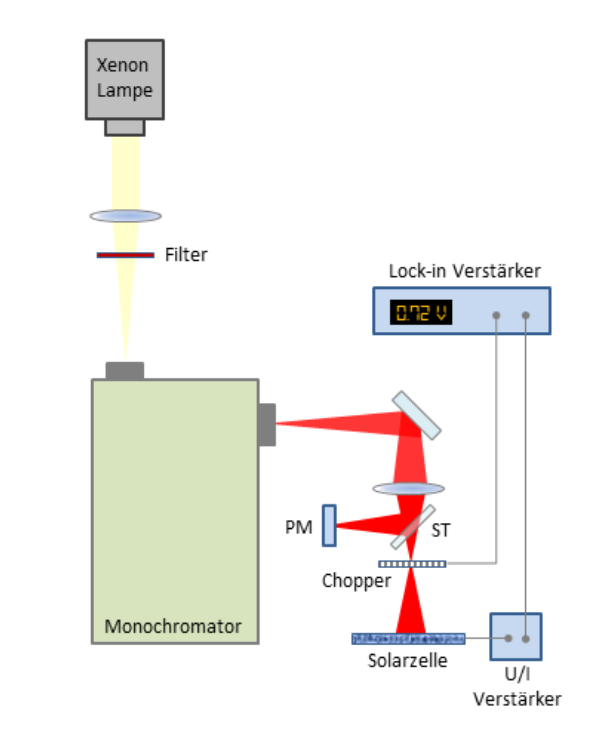
\includegraphics[]{Bilder/Versuchsaufbau1.png}
\end{figure}


